% answers.tex —— 2008 年·普通高等学校招生考试·浙江卷·文科 · 参考答案与详细解析片段
% 由 tools/generate_projects.py 依来源总账自 2008/2008_数学真题_浙江文_试题.md + 2008/2008_数学真题_浙江文_解析正文.md + 2008/2008_数学真题_浙江文_答案要点.md 生成，勿手改（改源 MD 后重跑）


\begin{gktip}
固定候选 PDF 仅含题面，无答案、解析和评分标准，原卷亦未标注分值；以下为非官方编者独立推导，官方答案字段为空。来源发布者、出版者、版次与官方身份均未核。
\end{gktip}

\begin{answer}
\gksolhead{1}{}

\textbf{题目}：

已知集合 $A=\{x\mid x>0\}$，$B=\{x\mid -1\leqslant x\leqslant2\}$，则 $A\cup B=$（　）

（A）$\{x\mid x\geqslant-1\}$

（B）$\{x\mid x\leqslant2\}$

（C）$\{x\mid 0<x\leqslant2\}$

（D）$\{x\mid -1\leqslant x\leqslant2\}$

\Needspace{4\baselineskip}
\textbf{解析}

\Needspace{5\baselineskip}
$A=(0,+\infty)$，$B=[-1,2]$，故

\nopagebreak[4]
\[A\cup B=[-1,+\infty)=\{x\mid x\geqslant-1\}.\]

\gkanswer{答案：A。}

\end{answer}
\begin{answer}
\gksolhead{2}{}

\textbf{题目}：

函数 $y=(\sin x+\cos x)^2+1$ 的最小正周期是（　）

（A）$\frac{\pi}2$

（B）$\pi$

（C）$\frac{3\pi}2$

（D）$2\pi$

\Needspace{4\baselineskip}
\textbf{解析}

\Needspace{5\baselineskip}
计算如下：

\nopagebreak[4]
\[y=(\sin x+\cos x)^2+1=1+\sin2x+1=2+\sin2x,\]

故最小正周期 $T=\dfrac{2\pi}2=\pi$。

\gkanswer{答案：B。}

\end{answer}
\begin{answer}
\gksolhead{3}{}

\textbf{题目}：

已知 $a$，$b$ 都是实数，那么“$a^2>b^2$”是“$a>b$”的（　）

（A）充分而不必要条件

（B）必要而不充分条件

（C）充分必要条件

（D）既不充分也不必要条件

\Needspace{4\baselineskip}
\textbf{解析}

$a^2>b^2$ 即 $|a|>|b|$。取 $a=-2$，$b=1$：$a^2>b^2$ 但 $a<b$，故不充分；取 $a=1$，$b=-2$：$a>b$ 但 $a^2<b^2$，故不必要。

\gkanswer{答案：D。}

\end{answer}
\begin{answer}
\gksolhead{4}{}

\textbf{题目}：

已知 $\{a_n\}$ 是等比数列，$a_2=2$，$a_5=\dfrac14$，则公比 $q=$（　）

（A）$-\frac12$

（B）$-2$

（C）$2$

（D）$\frac12$

\Needspace{4\baselineskip}
\textbf{解析}

\Needspace{5\baselineskip}
计算如下：

\nopagebreak[4]
\[q^3=\frac{a_5}{a_2}=\frac{1/4}2=\frac18\ \Longrightarrow\ q=\frac12.\]

\gkanswer{答案：D。}

\end{answer}
\begin{answer}
\gksolhead{5}{}

\textbf{题目}：

已知 $a\geqslant0$，$b\geqslant0$，且 $a+b=2$，则（　）

（A）$ab\leqslant\frac12$

（B）$ab\geqslant\frac12$

（C）$a^2+b^2\geqslant2$

（D）$a^2+b^2\leqslant3$

\Needspace{4\baselineskip}
\textbf{解析}

\Needspace{5\baselineskip}
由 $a+b=2$ 得 $ab\leqslant\left(\dfrac{a+b}2\right)^2=1$，故

\nopagebreak[4]
\[a^2+b^2=(a+b)^2-2ab=4-2ab\geqslant4-2=2,\]

等号在 $a=b=1$ 时成立。其余三项均可由 $a=2$，$b=0$ 或 $a=b=1$ 否定。

\gkanswer{答案：C。}

\end{answer}
\begin{answer}
\gksolhead{6}{}

\textbf{题目}：

在 $(x-1)(x-2)(x-3)(x-4)(x-5)$ 的展开式中，含 $x^4$ 的项的系数是（　）

（A）$-15$

（B）$85$

（C）$-120$

（D）$274$

\Needspace{4\baselineskip}
\textbf{解析}

\Needspace{5\baselineskip}
五个因式中取四个的 $x$、余下一个取常数，故 $x^4$ 的系数为

\nopagebreak[4]
\[-(1+2+3+4+5)=-15.\]

\gkanswer{答案：A。}

\end{answer}
\begin{answer}
\gksolhead{7}{}

\textbf{题目}：

在同一平面直角坐标系中，函数 $y=\cos\left(\dfrac x2+\dfrac{3\pi}2\right)$（$x\in[0,2\pi]$）的图象和直线 $y=\dfrac12$ 的交点个数是（　）

（A）$0$

（B）$1$

（C）$2$

（D）$4$

\Needspace{4\baselineskip}
\textbf{解析}

\Needspace{5\baselineskip}
计算如下：

\nopagebreak[4]
\[\cos\left(\frac x2+\frac{3\pi}2\right)=\sin\frac x2,\]

$x\in[0,2\pi]$ 时 $\dfrac x2\in[0,\pi]$，方程 $\sin\dfrac x2=\dfrac12$ 在 $[0,\pi]$ 内有两解 $\dfrac x2=\dfrac{\pi}6,\dfrac{5\pi}6$，即 $x=\dfrac{\pi}3,\dfrac{5\pi}3$。

\gkanswer{答案：C。}

\end{answer}
\begin{answer}
\gksolhead{8}{}

\textbf{题目}：

若双曲线 $\dfrac{x^2}{a^2}-\dfrac{y^2}{b^2}=1$ 的两个焦点到一条准线的距离之比为 $3:2$，则双曲线的离心率是（　）

（A）$3$

（B）$5$

（C）$\sqrt3$

（D）$\sqrt5$

\Needspace{4\baselineskip}
\textbf{解析}

\Needspace{5\baselineskip}
取右准线 $x=\dfrac{a^2}c$，两焦点 $(\pm c,0)$ 到它的距离分别为 $c-\dfrac{a^2}c$ 与 $c+\dfrac{a^2}c$，故

\nopagebreak[4]
\[\frac{c+\dfrac{a^2}c}{c-\dfrac{a^2}c}=\frac32\ \Longrightarrow\ 2\left(c^2+a^2\right)=3\left(c^2-a^2\right)\ \Longrightarrow\ c^2=5a^2,\]

故 $e=\dfrac ca=\sqrt5$。

\gkanswer{答案：D。}

\end{answer}
\begin{answer}
\gksolhead{9}{}

\textbf{题目}：

对两条不相交的空间直线 $a$ 与 $b$，必存在平面 $\alpha$，使得（　）

（A）$a\subset\alpha$，$b\subset\alpha$

（B）$a\subset\alpha$，$b\parallel\alpha$

（C）$a\perp\alpha$，$b\perp\alpha$

（D）$a\subset\alpha$，$b\perp\alpha$

\Needspace{4\baselineskip}
\textbf{解析}

取平面 $\alpha$ 经过 $a$ 且平行于 $b$（$a$，$b$ 不相交，方向确定，这样的平面存在），则 $a\subset\alpha$，$b\parallel\alpha$。其余三项在 $a$，$b$ 异面时均不成立。

\gkanswer{答案：B。}

\end{answer}
\begin{answer}
\gksolhead{10}{}

\textbf{题目}：

若 $a\geqslant0$，$b\geqslant0$，且当 $\begin{cases}x\geqslant0,\\ y\geqslant0,\\ x+y\leqslant1\end{cases}$ 时，恒有 $ax+by\leqslant1$，则以 $a$，$b$ 为坐标的点 $P(a,b)$ 所形成的平面区域的面积是（　）

（A）$\frac12$

（B）$\frac{\pi}4$

（C）$1$

（D）$\frac{\pi}2$

\Needspace{4\baselineskip}
\textbf{解析}

对固定的 $a$，$b\geqslant0$，$ax+by$ 在三角形（顶点 $(0,0)$，$(1,0)$，$(0,1)$）上的最大值为 $\max\{a,b\}$。故条件等价于 $a\leqslant1$ 且 $b\leqslant1$，即 $P(a,b)$ 构成边长为 $1$ 的正方形，面积为 $1$。

\gkanswer{答案：C。}

\end{answer}
\begin{answer}
\gksolhead{11}{}

\textbf{题目}：

已知函数 $f(x)=x^2+|x-2|$，则 $f(1)=$\gkblank{}。

\Needspace{4\baselineskip}
\textbf{解析}

\Needspace{5\baselineskip}
计算如下：

\nopagebreak[4]
\[f(1)=1+|1-2|=1+1=2.\]

\gkanswer{答案：$2$。}

\end{answer}
\begin{answer}
\gksolhead{12}{}

\textbf{题目}：

若 $\sin\left(\dfrac{\pi}2+\theta\right)=\dfrac35$，则 $\cos2\theta=$\gkblank{}。

\Needspace{4\baselineskip}
\textbf{解析}

\Needspace{5\baselineskip}
计算如下：

\nopagebreak[4]
\[\sin\left(\frac{\pi}2+\theta\right)=\cos\theta=\frac35,\]

\nopagebreak[4]
\[\cos2\theta=2\cos^2\theta-1=2\cdot\frac9{25}-1=-\frac7{25}.\]

\gkanswer{答案：$-\dfrac7{25}$。}

\end{answer}
\begin{answer}
\gksolhead{13}{}

\textbf{题目}：

已知 $F_1$，$F_2$ 为椭圆 $\dfrac{x^2}{25}+\dfrac{y^2}9=1$ 的两个焦点，过 $F_1$ 的直线交椭圆于 $A$，$B$ 两点。若 $|F_2A|+|F_2B|=12$，则 $|AB|=$\gkblank{}。

\Needspace{4\baselineskip}
\textbf{解析}

\Needspace{5\baselineskip}
由椭圆定义 $|AF_1|+|AF_2|=|BF_1|+|BF_2|=2a=10$，两式相加：

\nopagebreak[4]
\[\left(|AF_1|+|BF_1|\right)+\left(|AF_2|+|BF_2|\right)=20.\]

\Needspace{5\baselineskip}
已知 $|AF_2|+|BF_2|=12$，故 $|AF_1|+|BF_1|=8$。因 $A$，$F_1$，$B$ 共线且 $F_1$ 在 $A$，$B$ 之间，

\nopagebreak[4]
\[|AB|=|AF_1|+|BF_1|=8.\]

\gkanswer{答案：$8$。}

\end{answer}
\begin{answer}
\gksolhead{14}{}

\textbf{题目}：

在 $\triangle ABC$ 中，角 $A$，$B$，$C$ 所对的边分别为 $a$，$b$，$c$，若 $(\sqrt3b-c)\cos A=a\cos C$，则 $\cos A=$\gkblank{}。

\Needspace{4\baselineskip}
\textbf{解析}

\Needspace{5\baselineskip}
由射影定理 $a\cos C+c\cos A=b$，即 $a\cos C=b-c\cos A$。代入条件：

\nopagebreak[4]
\[(\sqrt3b-c)\cos A=b-c\cos A\ \Longrightarrow\ \sqrt3b\cos A=b\ \Longrightarrow\ \cos A=\frac{\sqrt3}3.\]

\gkanswer{答案：$\dfrac{\sqrt3}3$。}

\end{answer}
\begin{answer}
\gksolhead{15}{}

\textbf{题目}：

如图，已知球 $O$ 的面上四点 $A$，$B$，$C$，$D$，$DA\perp$ 平面 $ABC$，$AB\perp BC$，$DA=AB=BC=\sqrt3$，则球 $O$ 的体积等于\gkblank{}。
\nopagebreak[4]
\begin{center}% 2008 年浙江卷文科第 15 题：球 O 的面上四点 A、B、C、D，DA⊥平面 ABC，AB⊥BC，
%   DA=AB=BC=√3。
% 来源 PDF：gaokaomath-src/普通高考/2008/2008浙江文.pdf
% SHA-256：751204c132deb2b2...
% 原页：2008浙江文.pdf 第 1 页（A3 三栏）第 2 栏，书页码 493。
% 重绘依据：D 在 A 的正上方（DA 竖直），B 在 A 左下、C 在 B 左侧，AB⊥BC；
%   可见棱 DA、DB、DC、AB、BC 实线，被遮挡的底面斜边 CA 虚线。
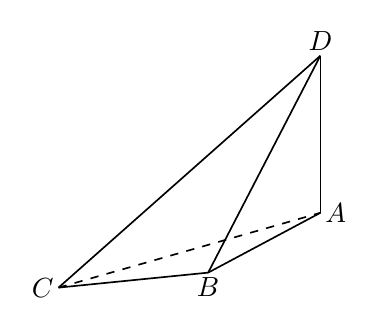
\begin{tikzpicture}[scale=0.95, semithick, every node/.style={inner sep=1.5pt}]
  \coordinate (D) at (5.0,4.7);
  \coordinate (A) at (5.0,2.6);
  \coordinate (B) at (3.5,1.8);
  \coordinate (C) at (1.5,1.6);

  \draw (D) -- (A);
  \draw (D) -- (B);
  \draw (D) -- (C);
  \draw (A) -- (B) -- (C);
  \draw[dashed] (C) -- (A);

  \node[above] at (D) {$D$};
  \node[right] at (A) {$A$};
  \node[below] at (B) {$B$};
  \node[left] at (C) {$C$};
\end{tikzpicture}
\end{center}
\nopagebreak[4]
\Needspace{4\baselineskip}
\textbf{解析}

\Needspace{5\baselineskip}
取坐标系使

\nopagebreak[4]
\[A(0,0,0),\quad B(\sqrt3,0,0),\quad C(\sqrt3,\sqrt3,0),\quad D(0,0,\sqrt3).\]

$\triangle ABC$ 在 $B$ 处为直角，外心为 $AC$ 中点 $M\left(\dfrac{\sqrt3}2,\dfrac{\sqrt3}2,0\right)$。

\Needspace{5\baselineskip}
球心在过 $M$ 且垂直于平面 $ABC$ 的直线上，设球心 $O'\left(\dfrac{\sqrt3}2,\dfrac{\sqrt3}2,h\right)$。由 $|O'A|=|O'D|$：

\nopagebreak[4]
\[h^2+\frac32=\frac32+(h-\sqrt3)^2\ \Longrightarrow\ h=\frac{\sqrt3}2,\]

\Needspace{5\baselineskip}
故

\nopagebreak[4]
\[R^2=h^2+\left(\frac{\sqrt3}2\right)^2+\left(\frac{\sqrt3}2\right)^2=\frac34+\frac32=\frac94,\qquad R=\frac32.\]

\nopagebreak[4]
\[V=\frac43\pi R^3=\frac43\pi\cdot\frac{27}8=\frac{9\pi}2.\]

\gkanswer{答案：$\dfrac{9\pi}2$。}

\end{answer}
\begin{answer}
\gksolhead{16}{}

\textbf{题目}：

已知 $\boldsymbol a$ 是平面内的单位向量，若向量 $\boldsymbol b$ 满足 $\boldsymbol b\cdot(\boldsymbol a-\boldsymbol b)=0$，则 $|\boldsymbol b|$ 的取值范围是\gkblank{}。

\Needspace{4\baselineskip}
\textbf{解析}

\Needspace{5\baselineskip}
设 $\boldsymbol a$，$\boldsymbol b$ 的夹角为 $\theta$，$|\boldsymbol a|=1$。由

\nopagebreak[4]
\[\boldsymbol b\cdot(\boldsymbol a-\boldsymbol b)=|\boldsymbol b|\cos\theta-|\boldsymbol b|^2=0\]

得 $|\boldsymbol b|=\cos\theta$，故 $0\leqslant|\boldsymbol b|\leqslant1$。

\gkanswer{答案：$[0,1]$。}

\end{answer}
\begin{answer}
\gksolhead{17}{}

\textbf{题目}：

用 $1,2,3,4,5,6$ 组成六位数（没有重复数字），要求任何相邻两个数字的奇偶性不同，且 $1$ 和 $2$ 相邻，这样的六位数的个数是\gkblank{}。（用数字作答）

\Needspace{4\baselineskip}
\textbf{解析}

相邻两数奇偶性不同，故六位数必为“奇偶奇偶奇偶”或“偶奇偶奇偶奇”两种模式之一。

\Needspace{5\baselineskip}
每种模式下，$1$ 只能占奇数位、$2$ 只能占偶数位，二者相邻的位置共有 $5$ 对（第 $1$—$2$、$2$—$3$、$\cdots$、$5$—$6$ 位），每对只有“$1$ 在前”一种填法；余下两个奇数与两个偶数分别任意排列，各 $2!$ 种。故每种模式有 $5\times2\times2=20$ 个，合计

\nopagebreak[4]
\[2\times20=40.\]

\gkanswer{答案：$40$。}

\end{answer}
\begin{answer}
\gksolhead{18}{}

\textbf{题目}：

已知数列 $\{x_n\}$ 的首项 $x_1=3$，通项 $x_n=2^np+nq$（$n\in\mathbf N^*$，$p$，$q$ 为常数），且 $x_1$，$x_4$，$x_5$ 成等差数列。求：

（1）$p$，$q$ 的值；

（2）数列 $\{x_n\}$ 前 $n$ 项和 $S_n$ 的公式。

\Needspace{4\baselineskip}
\textbf{解析}

\Needspace{5\baselineskip}
（1）$x_1=2p+q=3$；$x_4=16p+4q$，$x_5=32p+5q$。由 $x_1$，$x_4$，$x_5$ 成等差数列得

\nopagebreak[4]
\[2(16p+4q)=3+(32p+5q)\ \Longrightarrow\ 32p+8q=32p+5q+3\ \Longrightarrow\ q=1,\]

代回得 $p=1$。

\Needspace{5\baselineskip}
（2）$x_n=2^n+n$，故

\nopagebreak[4]
\[S_n=\sum_{k=1}^n\left(2^k+k\right)=\left(2^{n+1}-2\right)+\frac{n(n+1)}2.\]

\gkanswer{答案：（1）$p=1$，$q=1$；（2）$S_n=2^{n+1}-2+\dfrac{n(n+1)}2$。}

\end{answer}
\begin{answer}
\gksolhead{19}{}

\textbf{题目}：

一个袋中装有大小相同的黑球、白球和红球，已知袋中共有 $10$ 个球，从中任意摸出 $1$ 个球，得到黑球的概率是 $\dfrac25$；从中任意摸出 $2$ 个球，至少得到 $1$ 个白球的概率是 $\dfrac79$。求：

（1）从中任意摸出 $2$ 个球，得到的数是黑球的概率；

（2）袋中白球的个数。

\Needspace{4\baselineskip}
\textbf{解析}

\Needspace{5\baselineskip}
（1）由 $P(\text{\text{黑}})=\dfrac25$ 得黑球 $10\times\dfrac25=4$ 个。任取 $2$ 个都是黑球：

\nopagebreak[4]
\[P=\frac{\mathrm C_4^2}{\mathrm C_{10}^2}=\frac6{45}=\frac2{15}.\]

\Needspace{5\baselineskip}
（2）设白球 $w$ 个，则至少 $1$ 个白球的概率为 $1-\dfrac{\mathrm C_{10-w}^2}{\mathrm C_{10}^2}=\dfrac79$，故

\nopagebreak[4]
\[\frac{\mathrm C_{10-w}^2}{\mathrm C_{10}^2}=\frac29\ \Longrightarrow\ (10-w)(9-w)=20\ \Longrightarrow\ w^2-19w+70=0,\]

得 $w=5$ 或 $w=14$，由 $w\leqslant10$ 取 $w=5$。

【源疑点：原页第 (1) 问印作“从中任意摸出 $2$ 个球，得到的数是黑球的概率”，语句不通；按上下文与设问结构，应为“得到的两个球都是黑球的概率”。本库照原页转录题面，作答按“两个都是黑球”理解，特此说明。】

\gkanswer{答案：（1）$\dfrac2{15}$；（2）$5$。}

\end{answer}
\begin{answer}
\gksolhead{20}{}

\textbf{题目}：

如图，矩形 $ABCD$ 和梯形 $BEFC$ 所在平面互相垂直，$BE\parallel CF$，$\angle BCF=\angle CEF=90^\circ$，$AD=\sqrt3$，$EF=2$。

（1）求证：$AE\parallel$ 平面 $DCF$；

（2）当 $AB$ 的长为何值时，二面角 $A-EF-C$ 的大小为 $60^\circ$？
\nopagebreak[4]
\begin{center}% 2008 年浙江卷文科第 20 题：矩形 ABCD 与梯形 BEFC 所在平面互相垂直，BE∥CF，
%   ∠BCF=∠CEF=90°，AD=√3，EF=2。
% 来源 PDF：gaokaomath-src/普通高考/2008/2008浙江文.pdf
% SHA-256：751204c132deb2b2f856ffeba082ce94063aa6e279783c2f07e4cd84539ecb63
% 原页：2008浙江文.pdf 第 2 页（A3 三栏）第 1 栏，书页码 494。
% 重绘依据：按斜投影作图，保持 AB∥DC、AD∥BC、BE∥CF；A 左上、B 左下、D 右上、C 居中、
%   E 在中下、F 在右下；可见棱 AB、AD、AC、AE、AF、DF、BE、EF 实线，自 C 出发的
%   BC、CD、CE、CF 被遮挡用虚线。
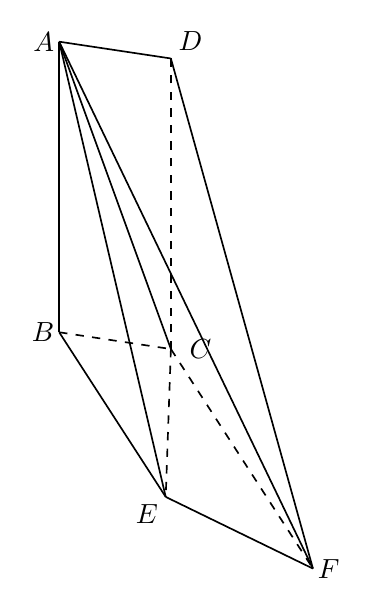
\begin{tikzpicture}[scale=0.82, semithick, every node/.style={inner sep=1.5pt}]
  \coordinate (A) at (1.00,8.50);
  \coordinate (B) at (1.00,4.00);
  \coordinate (C) at (2.73,3.74);
  \coordinate (D) at (2.73,8.24);
  \coordinate (E) at (2.65,1.45);
  \coordinate (F) at (4.93,0.34);

  % 可见棱
  \draw (A) -- (B);
  \draw (A) -- (D);
  \draw (A) -- (C);
  \draw (A) -- (E);
  \draw (A) -- (F);
  \draw (D) -- (F);
  \draw (B) -- (E);
  \draw (E) -- (F);

  % 被遮挡的棱（自 C 出发）
  \draw[dashed] (B) -- (C);
  \draw[dashed] (C) -- (D);
  \draw[dashed] (C) -- (E);
  \draw[dashed] (C) -- (F);

  \node[left] at (A) {$A$};
  \node[left] at (B) {$B$};
  \node[right=5pt] at (C) {$C$};
  \node[above right=1pt] at (D) {$D$};
  \node[below left=1pt] at (E) {$E$};
  \node[right] at (F) {$F$};
\end{tikzpicture}
\end{center}
\nopagebreak[4]
\Needspace{4\baselineskip}
\textbf{解析}

（1）取 $B$ 为原点，$BC$ 所在直线为 $y$ 轴，平面 $ABCD$ 为 $z=0$ 平面（$AB$ 沿 $x$ 轴），则平面 $BEFC$ 为 $x=0$ 平面。

$AD=BC=\sqrt3$，设 $AB=a$，则 $A(a,0,0)$，$D(a,\sqrt3,0)$，$C(0,\sqrt3,0)$。由 $BE\parallel CF$ 且 $\angle BCF=90^\circ$ 知 $BE$，$CF$ 都垂直于 $BC$，即都沿 $z$ 轴方向：$E(0,0,s)$，$F(0,\sqrt3,t)$。

\Needspace{5\baselineskip}
由 $\angle CEF=90^\circ$ 与 $EF=2$：

\nopagebreak[4]
\[\overrightarrow{CE}=(0,-\sqrt3,s),\quad \overrightarrow{EF}=(0,\sqrt3,t-s),\]

\nopagebreak[4]
\[\overrightarrow{CE}\cdot\overrightarrow{EF}=-3+s(t-s)=0,\qquad 3+(t-s)^2=4.\]

取 $t-s=1$，则 $s=3$，$t=4$，即 $E(0,0,3)$，$F(0,\sqrt3,4)$。

平面 $DCF$ 过 $D$，$C$，$F$，三点的 $y$ 坐标都是 $\sqrt3$，故平面 $DCF$ 为 $y=\sqrt3$；而 $\overrightarrow{AE}=(-a,0,3)$ 的 $y$ 分量为 $0$，且 $A$ 不在该平面内，故 $AE\parallel$ 平面 $DCF$。

（2）平面 $CEF$ 即 $x=0$，法向量 $\boldsymbol n_1=(1,0,0)$。

\Needspace{5\baselineskip}
平面 $AEF$ 中 $\overrightarrow{AE}=(-a,0,3)$，$\overrightarrow{AF}=(-a,\sqrt3,4)$，法向量

\nopagebreak[4]
\[\boldsymbol n_2=\overrightarrow{AE}\times\overrightarrow{AF}=\left(-3\sqrt3,\ a,\ -a\sqrt3\right),\qquad |\boldsymbol n_2|=\sqrt{27+4a^2}.\]

\Needspace{5\baselineskip}
由二面角为 $60^\circ$：

\nopagebreak[4]
\[\frac{\left|\boldsymbol n_1\cdot\boldsymbol n_2\right|}{|\boldsymbol n_1||\boldsymbol n_2|}=\frac{3\sqrt3}{\sqrt{27+4a^2}}=\frac12\ \Longrightarrow\ 27+4a^2=108\ \Longrightarrow\ a=\frac92,\]

即 $AB=\dfrac92$。

\gkanswer{答案：（1）证明见解析；（2）$AB=\dfrac92$。}

\end{answer}
\begin{answer}
\gksolhead{21}{}

\textbf{题目}：

已知 $a$ 是实数，函数 $f(x)=x^2(x-a)$。

（1）若 $f'(1)=3$，求 $a$ 的值及曲线 $y=f(x)$ 在点 $(1,f(1))$ 处的切线方程；

（2）求 $f(x)$ 在区间 $[0,2]$ 上的最大值。

\Needspace{4\baselineskip}
\textbf{解析}

\Needspace{5\baselineskip}
（1）$f(x)=x^3-ax^2$，$f'(x)=3x^2-2ax$。由 $f'(1)=3-2a=3$ 得 $a=0$，此时 $f(x)=x^3$，$f(1)=1$，切线

\nopagebreak[4]
\[y-1=3(x-1),\qquad\text{\text{即} }y=3x-2.\]

（2）$f'(x)=x(3x-2a)$，$[0,2]$ 上的驻点为 $x=\dfrac{2a}3$（当 $0<\dfrac{2a}3<2$ 时）。

\begin{itemize}
\item 若 $a<0$，则 $\dfrac{2a}3<0$，$f'(x)\geqslant0$，$f$ 在 $[0,2]$ 上递增，最大值为 $f(2)=8-4a$。
\item 若 $0\leqslant a<2$，则 $0\leqslant\dfrac{2a}3<\dfrac43<2$，$f$ 在 $\left[0,\dfrac{2a}3\right]$ 上递减、在 $\left[\dfrac{2a}3,2\right]$ 上递增，最大值为 $\max\{f(0),f(2)\}=\max\{0,8-4a\}=8-4a$。
\item 若 $a\geqslant2$，则 $f(2)=8-4a\leqslant0=f(0)$，且 $f$ 在 $\left[\dfrac{2a}3,2\right]$ 上递增，最大值为 $f(0)=0$。
\end{itemize}

综上：$a<2$ 时最大值为 $8-4a$；$a\geqslant2$ 时最大值为 $0$。

\gkanswer{答案：（1）$a=0$，$y=3x-2$；（2）$a<2$ 时最大值 $8-4a$，$a\geqslant2$ 时最大值 $0$。}

\end{answer}